\section{Learning Node Embeddings}
Following \cite{node-emb-latent-space}, we project nodes into a latent space and the geometric relations in that space correspond to those in the original graph.
\begin{marginfigure}
	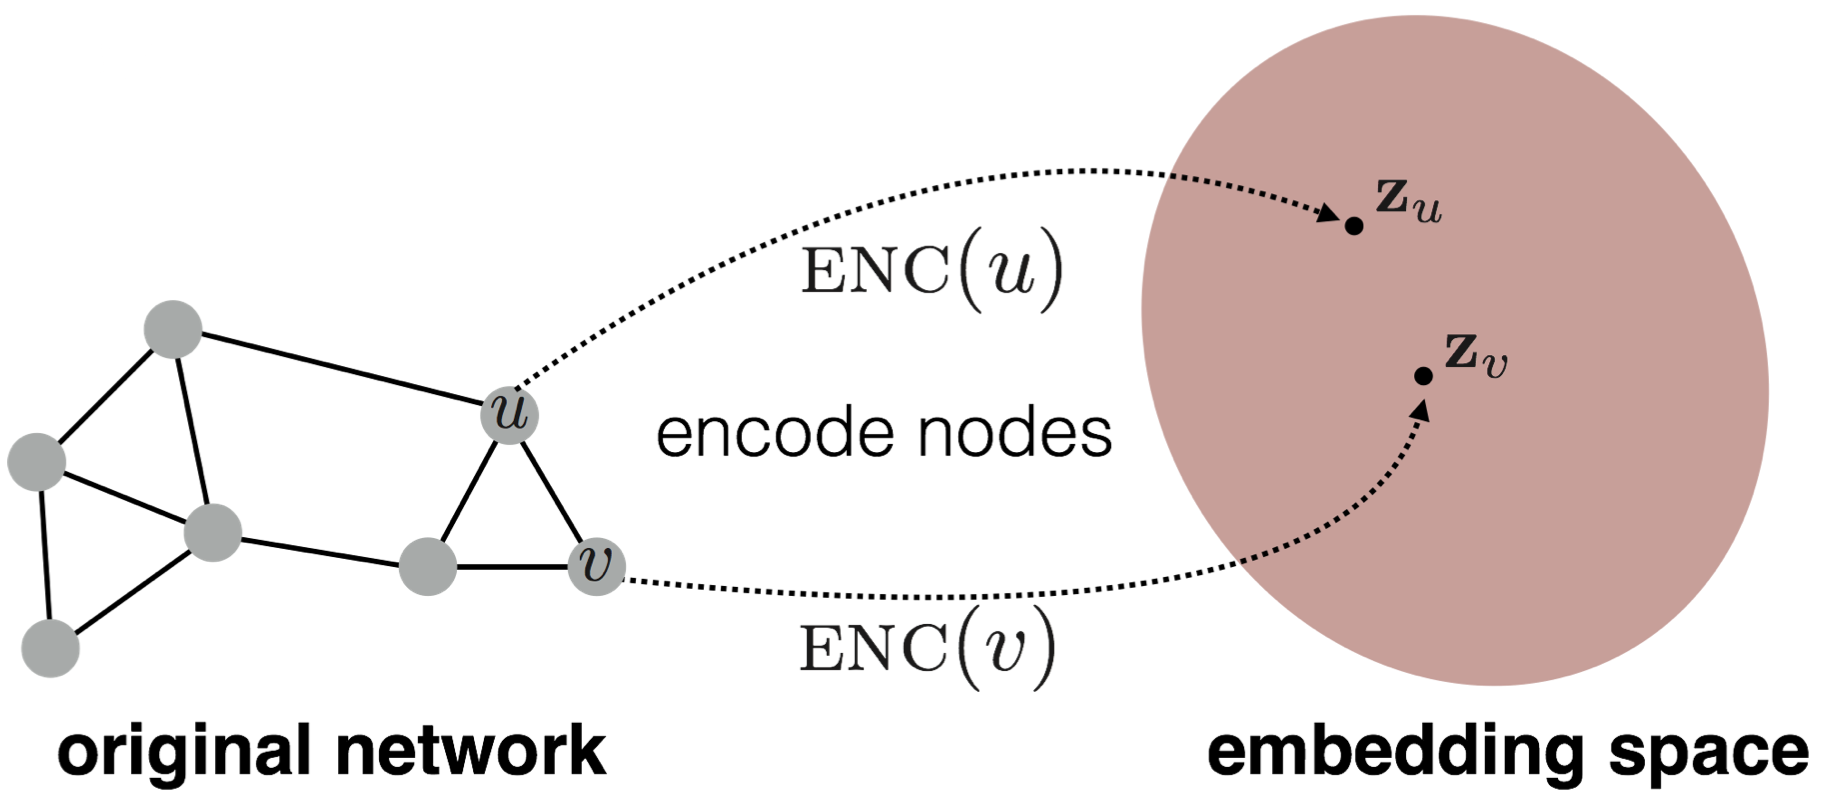
\includegraphics[width=\textwidth]{node-embeddings.png}
	\caption{Node Representation Learning Source: \href{https://snap-stanford.github.io/cs224w-notes/machine-learning-with-networks/node-representation-learning}{Stanford}}
	\label{fig:node-embedding}
\end{marginfigure}
\subsection{Encoder-Decoder Model}
The task is essentially to \textit{encode} each node into a low-dimensional vector, and finally \textit{decode} the embedding and use it to reconstruct information \cite{representation-learning-methods}.
\begin{definition}[Encoder]
The encoder is a function \texttt{ENC}$:V \to \mathbb{R}^d$ which maps nodes $v \in V$ to vector embeddings $\mathbf{z}_v \in \mathbb{R}^d$.. Commonly the approach is a shallow embedding one, and thus the encoder function is an embedding lookup on the node ID, i.e \texttt{ENC}$(v) = \mathbf{Z}[v]$ where $\mathbf{Z} \in \mathbb{R}^{|V| \times d}$ is the embedding matrix.
\end{definition}
\begin{definition}[Decoder]
The decoder reconstructs certain graph statistics from node embeddings generated by the encoder. It is common to use pairwise decoders, i.e \texttt{DEC}$:\mathbb{R}^d \times \mathbb{R}^d \to \mathbb{R}^+$ and they are similarity measures.
\end{definition}
The goal is to minimize reconstruction loss, i.e 
\begin{equation}\label{eq:recon-loss}
\texttt{DEC}(\texttt{ENC}(u), \texttt{ENC}(v)) = \texttt{DEC}(\mathbf{z}_u, \mathbf{z}_v) \approx \mathbf{S}[u, v]
\end{equation}
\marginnote{
	Mean Squared Error loss:
	\begin{equation*}
		MSE(y, \tilde{y}) = \dfrac{1}{n}\sum_{i=1}^n (y_i - \tilde{y}_i)^2
	\end{equation*}
	Cross Entropy loss:
	\begin{equation*}
		CE(y, \tilde{y}) = -\dfrac{1}{n}\sum_{i=1}^n y_i \log(\tilde{y}_i)
	\end{equation*}
}
To achieve the goal above, we minimize an empirical reconstruction loss function
\begin{equation}
\mathcal{L} = \sum_{(u, v) \in \mathcal{D}} \ell(\texttt{DEC}(\mathbf{z}_u, \mathbf{z}_v), \mathbf{S}[u,v])
\end{equation}
\noindent where $\mathcal{D}$ is a subset of node pairs, and $\ell$ is a loss function such as cross-entropy or mean-squared error loss. We look at some common shallow embedding algorithms:
\begin{enumerate}
\item \textbf{Factorization based Encoder-Decoder}\\
The loss function for such approaches can be minimized using factorization algorithms such as SVD.
\begin{enumerate}
\item \textbf{Laplacian Eigenmaps} \cite{laplacian-eigenmaps}: 
	\marginnote{If we construct $\mathbf{S}$ to satisfy properties of $\mathbf{L}$, and $\mathbf{z}_u$ are $d$-dimensional, then the optimal solution for minimizing the loss is given by the $d$ smallest eigenvectors of $\mathbf{L}$ excluding the smallest one, i.e $\mathbf{1}$}
It is an old but influential approach built upon spectral clustering. The decoder is 
\begin{equation}
	\texttt{DEC}(\mathbf{z}_u, \mathbf{z}_v) = ||\mathbf{z}_u - \mathbf{z}_v||_2^2
\end{equation}
and the loss function is
 \begin{equation}
\mathcal{L} = \sum_{(u,v) \in \mathcal{D}} \texttt{DEC}(\mathbf{z}_u, \mathbf{z}_v)\mathbf{S}[u,v]
\end{equation}
\item \textbf{Inner-product methods}: The decoder in these is 
\begin{equation}
\texttt{DEC}(\mathbf{z}_u, \mathbf{z}_v) = \mathbf{z}_u^T\mathbf{z}_v
\end{equation}
and the loss function is
\begin{equation}
\mathcal{L} = \sum_{(u,v) \in \mathcal{D}} ||\texttt{DEC}(\mathbf{z}_u, \mathbf{z}_v) - \mathbf{S}[u,v]||_2^2
\end{equation}

\begin{enumerate}
	\item \textit{Graph Factorization} \cite{graph-factorization}: It uses $\mathbf{S} \triangleq \mathbf{A}$.
	\item \textit{GraRep} \cite{grarep}: It defines $\mathbf{S}$ based on powers of $\mathbf{A}$.
	\item \textit{HOPE} \cite{hope}: It defines $\mathbf{S}$ based on neighborhood overlap measures.
\end{enumerate}
\end{enumerate}
\item \textbf{Random Walk Embeddings} \\
The notion in such embeddings are that two nodes have similar embeddings if they tend to co-occur on short random walks over the graph. We learn embeddings to get
\begin{equation} \label{eq:random-walk-decoder}
\texttt{DEC}(\mathbf{z}_u, \mathbf{z}_v) \triangleq \dfrac{e^{\mathbf{z}_u^T \mathbf{z}_v}}{\sum_{w \in V} e^{\mathbf{z}_u^T \mathbf{z}_w}} \approx p_{G, T}(v|u)
\end{equation}
\marginnote{The notation $\Iintv{x,y}$ denotes the integer interval spanning from $x$ to $y$, i.e $\{x, \cdots y\}$}
where $p_{G,T}(v|u)$ is the probability of reaching node $v$ starting at $u$ on a $T$-length random walk ($T \in \Iintv{2, 10}$). Clearly the decoder is learning an asymmetric stochastic measure. To train the embeddings, the loss function employed is
\begin{equation}
\mathcal{L} = \sum_{(u,v) \in \mathcal{D}} -\log(\texttt{DEC}(\mathbf{z}_u, \mathbf{z}_v))
\end{equation}
	\marginnote{It has been shown in \cite{network-embedding-matrix} that if we define 
	\begin{equation*}
		\mathbf{S}_{DW} = \log\bigg(\dfrac{\sum_{w \in V}d_w}{T} \Big(\sum_{t=1}^T\mathbf{P}^t\Big)\mathbf{D}^{-1}\bigg) - \log (b)
	\end{equation*}
	then, the embeddings $\mathbf{Z}$ by DeepWalk satisfy $\mathbf{Z}^T \mathbf{Z} \approx \mathbf{S}_{DW}$. What is interesting to note that is we can eigendecompose the interior of above equation, and note that DeepWalk is closely related to $\mathbf{L}_{sym}$ and hence spectral clustering, but differ by the fact that influence of eigenvalues is controlled by DeepWalk through $T$.
}
But the issue here is that evaluating the loss function has time complexity $\mathcal{O}(|V||\mathcal{D}|) \sim \mathcal{O}(|V|^2)$.
\begin{enumerate}
	\item \textbf{DeepWalk} \cite{deepwalk}: 
	It employs uniformly random walks to define $p_{G,T}(v|u)$ and employs hierarchical softmax \cite{hierarchical-softmax} to approximate Equation (\ref{eq:random-walk-decoder})
	\item \textbf{node2vec} \cite{node2vec}: It introduces hyperparameters to allow random walk probabilities to interpolate between walks more akin to BFS or DFS. It uses noise contrastive estimation along with negative sampling to rewrite $\mathcal{L}$ as
	\begin{equation}
	\mathcal{L} = \sum_{(u,v)\in\mathcal{D}} -\log(\sigma(\mathbf{z}_u^T\mathbf{z}_v)) - \gamma \mathbb{E}_{v_n \sim P_n(V)}[\log(-\sigma(\mathbf{z}_u^T \mathbf{z_{v_n}}))]
	\end{equation}
	with $\gamma > 0$ and $P_n(V)$ being the uniform distribution. Monte Carlo Sampling is used to calculate the expectation.
	\item \textbf{LINE} \cite{line}: It proposes a first objective
	\begin{equation}
		\texttt{DEC}(\mathbf{z}_u, \mathbf{z}_v) = \sigma(\mathbf{z}_u^T\mathbf{z}_v)
	\end{equation}
\marginnote{
\textbf{KL-Divergence}
\begin{equation*}
	D_{KL}(p \parallel q) = \sum_{i=1}^n p(x_i) \log\bigg(\dfrac{p(x_i)}{q(x_i)}\bigg)
\end{equation*}
}
and $\mathbf{S}[u,v] = A_{uv}$. Along with that, a second objective is the decoder same as DeepWalk, but trained using KL-Divergence to encode 2-hop information (i.e $\mathbf{A}^2$), and it explicitly reconstructs first and second-order neighborhood information.
\end{enumerate}
\end{enumerate}
\subsection{Drawbacks of Shallow Embeddings}
\begin{itemize}
	\item[$\diamond$] Lack of parameter sharing between nodes is a hinder to statistic and computational efficiency. We want embeddings to be independent of $|V|$.
	\item[$\diamond$] They do not leverage node features in \texttt{ENC}.
	\item[$\diamond$] They are transductive, and thus it is difficult to generate embeddings for newer nodes and cannot be used in inductive applications which involve generalization.
\end{itemize}
\marginnote{\textbf{Knowledge Graphs}: They are multi-relational graphs $G = (V,E)$ with edges defined as tuples $e = (u, \tau, v)$ indicating the presence of a relation $\tau \in \mathcal{R}$ between two nodes. The task of knowledge graph completion is generally to predict the missing edges in the graph.}
\subsection{Reconstruction of Multi-Relational Data}
Multi-relational graphs add a relation type, and to address that, we make the decoder multi-relational, i.e $\texttt{DEC}: \mathbb{R}^d \times \mathcal{R} \times \mathbb{R}^d \to \mathbb{R}^+$.
\textbf{RESCAL} \cite{rescal} defines the multi-relational decoder as $\texttt{DEC}(u, \tau, v) = \mathbf{z}_u^T \mathbf{R}_\tau \mathbf{z}_v$, where $\mathbf{R}_\tau$ is a learnable matrix for relation $\tau \in \mathcal{R}$, and we can learn $\mathbf{Z}$ and $\mathbf{R}_\tau$ using a simple reconstruction loss 
\begin{equation} \label{eq:mr-recon-loss}
\mathcal{L} = \sum_{u\in V} \sum_{v\in V} \sum_{\tau \in \mathcal{R}} ||\mathbf{z}_u^T \mathbf{R}_\tau \mathbf{z}_v - \mathcal{A}_{u\tau v}||^2]
\end{equation}
As seen above, it is a common practice to define the similarity measure based on the adjacency tensor, and thus we are trying to reconstruct immediate neighbors from the embeddings. \\
\begin{enumerate}
\item \textbf{Loss Functions}: The loss defined in Equation (\ref{eq:mr-recon-loss}) requires $\mathcal{O}(|V|^2|\mathcal{R}|)$ time complexity, and is extremely expensive. Since it is realistically seen that multi-relational graphs are sparse, we would want a loss function of the order $\mathcal{O}(|E|)$. Also, since our target is to decode the adjacency tensor, which has binary values, we can't use the simple MSE loss.
\begin{enumerate}
	\item \textbf{Cross-Entropy with Negative Sampling}: Defining $\sigma$ as the sigmoid function, $P_{n,u}(V)$ as the negative sampling distribution, and $\gamma > 0$, we write
	\begin{equation}
	\begin{split}
	\mathcal{L} = \sum_{(u, \tau, v) \in E}\bigg(& -\log(\sigma(\texttt{DEC}(\mathbf{z}_u, \tau, \mathbf{z}_v))) \\&- \gamma \mathbb{E}_{v_n \sim P_{n, u}(V)}[\log(\sigma(-\texttt{DEC}(\mathbf{z}_u, \tau, \mathbf{z}_{v_n})))] \bigg)
	\end{split}
	\end{equation}
If we calculate the expectation using Monte Carlo Sampling, we can write by sampling over a small subet $\mathcal{P}_{n,u} \subset P_{n,u}(V)$
\begin{equation}
\mathcal{L} = -\sum_{(u, \tau, v) \in E}\log(\sigma(\texttt{DEC}(\mathbf{z}_u, \tau, \mathbf{z}_v)))	- \sum_{v_n \in \mathcal{P}_{n, u}}\log(\sigma(-\texttt{DEC}(\mathbf{z}_u, \tau, \mathbf{z}_{v_n})))
\end{equation}
	\item \textbf{Max-Margin Loss}: Also called the \textit{hinge loss}, we set a margin $\Delta$ and use \textit{contrastive estimation} (but with direct comparison of output of the decoders) to write the loss function as
	\begin{equation}
		\mathcal{L} = \sum_{(u, \tau, v) \in E} \sum_{v_n \in \mathcal{P}_{n, u}} \max(0, -\texttt{DEC}(\mathbf{z}_u, \tau, \mathbf{z}_v) + \texttt{DEC}(\mathbf{z}_u, \tau, \mathbf{z}_{v_n}) + \Delta)
	\end{equation}
\end{enumerate}
\item \textbf{Decoders}:
\begin{enumerate}
	\item \textbf{RESCAL}: In the RESCAL decoder, a trainable matrix $\mathbf{R}_\tau \in \mathbb{R}^{d \times d}$ is associated with each relation
	\begin{equation}
		\texttt{DEC}(\mathbf{z}_u, \tau, \mathbf{z}_v) = \mathbf{z}_u^T \mathbf{R}_\tau \mathbf{z}_v
	\end{equation}
	 This gives rise to $\mathcal{O}(d^2)$ number of parameters for each relation, and that has high computational cost. Recent decoders aim to get $\mathcal{O}(d)$ number of parameters.
	 \item \textbf{Translational Decoders}: Such decoders represent relations as translations in embedding space. 
	 \begin{enumerate}
	 	\item \textbf{TransE} \cite{transe}: Using a $d$-dimensional embedding, the decoder is
	 	\begin{equation}
	 		\texttt{DEC}(\mathbf{z}_u, \tau, \mathbf{z}_v) = -||\mathbf{z}_u + \mathbf{r}_\tau - \mathbf{z}_v||
	 	\end{equation}
 	It is a simple decoder, and the likelihood of an edge is proportional to the distance translated according to the relation.
 	\item \textbf{TransX}: These are a class of models built upon the TransE model, and have the general form
 	\begin{equation}
 		\texttt{DEC}(\mathbf{z}_u, \tau, \mathbf{z}_v) = -||g_{1, \tau}(\mathbf{z}_u) + \mathbf{r}_\tau - g_{2,\tau}(\mathbf{z}_v)||
 	\end{equation}
 where $g_{i,\tau}$ are trainable transformations. \cite{transh} proposed the TransH model which projects the entity embeddings onto a learnable relation-specific hyperplane defined by the normal vector $\mathbf{w}_r$ and then translating it.
 \begin{equation}
 	\texttt{DEC}(\mathbf{z}_u, \tau, \mathbf{z}_v) = -||(\mathbf{z}_u - \mathbf{w}_r^T \mathbf{z}_u \mathbf{w}_r) + \mathbf{r}_\tau - (\mathbf{z}_v - \mathbf{w}_r^T \mathbf{z}_v \mathbf{w}_r)||
 \end{equation}
	 \end{enumerate}
 \item \textbf{DistMult} \cite{distmult}: This generalizes the dot-product decoder from simple graphs, thus
 \begin{equation}
 	\texttt{DEC}(\mathbf{z}_u, \tau, \mathbf{z}_v) = \langle \mathbf{z}_u, \mathbf{r}_\tau, \mathbf{z}_v \rangle = \sum_{i=1}^d \mathbf{z}_u[i] \times \mathbf{r}_\tau[i] \times \mathbf{z}_v[i]
 \end{equation}
This has a restriction, that it can only be used for symmetric relations, but majority of the relation are assymetric.
\item \textbf{ComplEx} \cite{complex}: This extends the above idea and uses complex-valued embeddings, to bring in asymmetry, i.e $\mathbf{z}_u, \mathbf{r}_\tau, \mathbf{z}_v \in \mathbb{C}^d$.
 \begin{equation}
	\texttt{DEC}(\mathbf{z}_u, \tau, \mathbf{z}_v) = \Re\langle \mathbf{z}_u, \mathbf{r}_\tau, \bar{\mathbf{z}}_v \rangle =\Re\bigg( \sum_{i=1}^d \mathbf{z}_u[i] \times \mathbf{r}_\tau[i] \times \bar{\mathbf{z}}_v[i]\bigg)
\end{equation}
\item \textbf{RotatE} \cite{rotate}: This is again a complex-valued decoder, with the constraint that $|\mathbf{r}_\tau[i]| = 1 \implies \mathbf{r}_\tau[i] =e^{\iota \theta_{r, i}}$. This brings in rotations in the complex plane, and 
\begin{equation}
	\texttt{DEC}(\mathbf{z}_u, \tau, \mathbf{z}_v) = - || \mathbf{z}_u \circ \mathbf{r}_\tau - \mathbf{z}_v||
\end{equation}
\end{enumerate}
\end{enumerate}
\subsection{Representation Abilities of Multi-Relational Decoders}
We characterize the representation abilities of the multi-relational decoders in three ways:
\marginnote{Symmetric relations mean that \[ (u, \tau, v) \in E \leftrightarrow (v, \tau, u) \in E\]
Anti-symmetric relations mean that \[ (u, \tau, v) \in E \rightarrow (v, \tau, u) \notin E\]}
\begin{itemize}
	\item[$\diamond$] \textbf{Symmetry}: Can different decoders model both symmetric and anti-symmetric relations? DistMult can only model symmetric, while TransE can only model anti-symmetric, while all others are seen to model both.
	\marginnote{Inversion means that \[ (u, \tau_1, v) \in E\leftrightarrow (v, \tau_2, u) \in E\]}
	\item[$\diamond$] \textbf{Inversion}: Most decoders can model inversion, though TransX and DistMult fail in this respect.
	\marginnote{Compositionality means that \[(u, \tau_1, y) \in E \land (y, \tau_2, v) \in E \rightarrow (u, \tau_3, v) \in E\]}
	\item[$\diamond$] \textbf{Compositionality}: It is seen that in RESCAL, defining $\mathbf{R}_{\tau_3} = \mathbf{R}_{\tau_1}\mathbf{R}_{\tau_2}$ and in TransE defining $\mathbf{r}_{\tau_3} = \mathbf{r}_{\tau_1} + \mathbf{r}_{\tau_2}$ allows modeling of compositionality. RotateE also models it, while the rest three decoders we saw fail to do so.
\end{itemize}